\chapter{Clustering}

\section{Clustering hiérarchique}
    Cette méthode, bien qu'utile quand on ne connaît pas le nombre de clusters
    attendu, ne passe pas à l'échelle~: son exécution sur la totalité du jeu de
    donnée provoque un dépassement de mémoire.

    Nous avons malgré tout réalisé un échantillonnage aléatoire (de 1,000 lignes)
    de notre jeu de données sur lequel on a effectué un \textit{clustering hiérarchique}
    afin d'avoir une idée sur le nombre de clusters qui pouvaient être extraits.

    \begin{figure}[h]
        \centering
        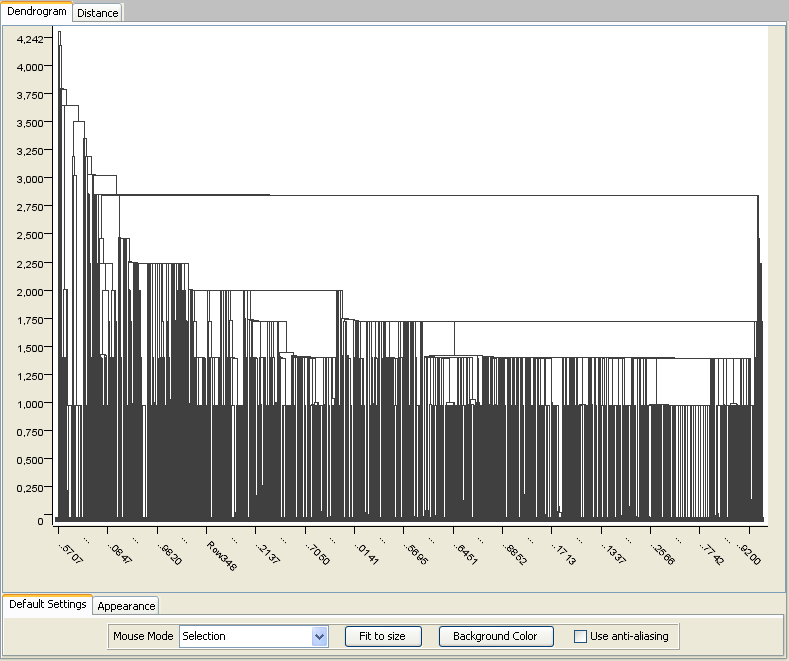
\includegraphics[scale=0.35]{../screenshots/hierarchical_clustering_1000_samples.png}
        \caption{R\'esultat du clusturing hiérarchique sur 1000 \'echantillons}
        \label{diagram:hierarchical_clustering_1000_samples}
    \end{figure}

    Mais même sur un jeu de données aussi restreint (par rapport aux données
    originales), le résultat était difficilement exploitable (car très dense),
    et le fait que les données exploitées représentaient moins de $5\%$ des
    données originales faisait que ce clustering était fort instable (structure
    variant sur des samplings différents).

\section{K-Means}


\section{DBScan}
